% This is the Reed College LaTeX thesis template. Most of the work
% for the document class was done by Sam Noble (SN), as well as this
% template. Later comments etc. by Ben Salzberg (BTS). Additional
% restructuring and APA support by Jess Youngberg (JY).
% Your comments and suggestions are more than welcome; please email
% them to cus@reed.edu
%
% See http://web.reed.edu/cis/help/latex.html for help. There are a
% great bunch of help pages there, with notes on
% getting started, bibtex, etc. Go there and read it if you're not
% already familiar with LaTeX.
%
% Any line that starts with a percent symbol is a comment.
% They won't show up in the document, and are useful for notes
% to yourself and explaining commands.
% Commenting also removes a line from the document;
% very handy for troubleshooting problems. -BTS

% As far as I know, this follows the requirements laid out in
% the 2002-2003 Senior Handbook. Ask a librarian to check the
% document before binding. -SN

%%
%% Preamble
%%
% \documentclass{<something>} must begin each LaTeX document
\documentclass[12pt,twoside]{reedthesis}
% Packages are extensions to the basic LaTeX functions. Whatever you
% want to typeset, there is probably a package out there for it.
% Chemistry (chemtex), screenplays, you name it.
% Check out CTAN to see: http://www.ctan.org/
%%
\usepackage{graphicx,latexsym}
\usepackage{amsmath}
\usepackage{amssymb,amsthm}
\usepackage{longtable,booktabs,setspace}
\usepackage{chemarr} %% Useful for one reaction arrow, useless if you're not a chem major
\usepackage[hyphens]{url}
% Added by CII
\usepackage{hyperref}
\usepackage{lmodern}
\usepackage{float}
\floatplacement{figure}{H}
% End of CII addition
\usepackage{rotating}

% Next line commented out by CII
%%% \usepackage{natbib}
% Comment out the natbib line above and uncomment the following two lines to use the new
% biblatex-chicago style, for Chicago A. Also make some changes at the end where the
% bibliography is included.
%\usepackage{biblatex-chicago}
%\bibliography{thesis}


% Added by CII (Thanks, Hadley!)
% Use ref for internal links
\renewcommand{\hyperref}[2][???]{\autoref{#1}}
\def\chapterautorefname{Chapter}
\def\sectionautorefname{Section}
\def\subsectionautorefname{Subsection}
% End of CII addition

% Added by CII
\usepackage{caption}
\captionsetup{width=5in}
% End of CII addition

% \usepackage{times} % other fonts are available like times, bookman, charter, palatino


% To pass between YAML and LaTeX the dollar signs are added by CII
\title{INFFOREST Variable Importance on Random Forests}
\author{Aurora Owens}
% The month and year that you submit your FINAL draft TO THE LIBRARY (May or December)
\date{May 2017}
\division{Mathematics and Natural Sciences}
\advisor{Andrew Bray}
%If you have two advisors for some reason, you can use the following
% Uncommented out by CII
% End of CII addition

%%% Remember to use the correct department!
\department{Mathematics}
% if you're writing a thesis in an interdisciplinary major,
% uncomment the line below and change the text as appropriate.
% check the Senior Handbook if unsure.
%\thedivisionof{The Established Interdisciplinary Committee for}
% if you want the approval page to say "Approved for the Committee",
% uncomment the next line
%\approvedforthe{Committee}

% Added by CII
%%% Copied from knitr
%% maxwidth is the original width if it's less than linewidth
%% otherwise use linewidth (to make sure the graphics do not exceed the margin)
\makeatletter
\def\maxwidth{ %
  \ifdim\Gin@nat@width>\linewidth
    \linewidth
  \else
    \Gin@nat@width
  \fi
}
\makeatother

\renewcommand{\contentsname}{Table of Contents}
% End of CII addition

\setlength{\parskip}{0pt}

% Added by CII

\providecommand{\tightlist}{%
  \setlength{\itemsep}{0pt}\setlength{\parskip}{0pt}}

\Acknowledgements{
I want to thank a few people.
}

\Dedication{
You can have a dedication here if you wish.
}

\Preface{
This is an example of a thesis setup to use the reed thesis document
class.
}

\Abstract{
The preface pretty much says it all. \par  Second paragraph of abstract
starts here.
}

	\usepackage{algorithm}
	\usepackage{algpseudocode}
	\usepackage{float}
% End of CII addition
%%
%% End Preamble
%%
%

\begin{document}

% Everything below added by CII
      \maketitle
  
  \frontmatter % this stuff will be roman-numbered
  \pagestyle{empty} % this removes page numbers from the frontmatter

      \begin{acknowledgements}
      I want to thank a few people.
    \end{acknowledgements}
  
      \begin{preface}
      This is an example of a thesis setup to use the reed thesis document
      class.
    \end{preface}
  
      \hypersetup{linkcolor=black}
    \setcounter{tocdepth}{2}
    \tableofcontents
  
      \listoftables
  
      \listoffigures
  
      \begin{abstract}
      The preface pretty much says it all. \par  Second paragraph of abstract
      starts here.
    \end{abstract}
  
      \begin{dedication}
      You can have a dedication here if you wish.
    \end{dedication}
  
  \mainmatter % here the regular arabic numbering starts
  \pagestyle{fancyplain} % turns page numbering back on

  \chapter{Introduction}\label{introduction}
  
  \section{Trees and Random Forests}\label{trees-and-random-forests}
  
  \subsection{Trees}\label{trees}
  
  ~~~~~Decision trees may be familiar to many with a background in social
  science as a convenient way to represent data and assist in decision
  making. Morgan and Sonquist (1963) derived a way for constructing trees
  motivated by the specific feature space of data collected from
  interviews and surveys. Unlike, agricultural data which involves mostly
  numeric variables, the data collected from interviews is mostly
  categorical. On top of this, the datasets Morgan and Sonquist dealt with
  had few participants, and a lot of data collected on each one. To add to
  their difficulties, there was reason to believe that there were lurking
  errors in the data that would be hard identify and quantify. Lastly,
  many of the predictors were correlated. Morgan and Sonquist doubted that
  the additive assumptions of many models would be appropriate for this
  data. They noted that while many statistical methods would have
  difficulty accurately parsing this data, a clever researcher with quite
  a lot of time could create a suitable model simply by grouping values in
  the feature space and predicting that the response corresponding to
  these values would be an average of the observed responses given the
  grouped conditions. Their formalization of this procedure in terms of
  ``decision rules'' laid the ground work for future research on decision
  trees.
  
  ~~~~~Later researchers proposed new methods for creating trees that
  improved upon the Morgan and Sonquist model. Leo Breiman et al (1984)
  proposed an algorithm called CART, \emph{classification and regression
  trees}, that would allow trees to be fit on various types of data. An
  alternative to this method is conditional inference trees. Torsten
  Hothorn, Kurt Hornik, Achim Zeileis argue in their 2006 paper
  \emph{Unbiased Recursive Partitioning: A Conditional Inference
  Framework}, CART has a selection bias toward variables with either
  missing values or a great number of possible splits. This bias can
  effect the interpretability of all tree models fit using this method. As
  an alternative to CART and other algorithms, Hothorn et al propose a new
  method, conditional inference trees.
  
  ~~~~~ There is a limit to the predictive capabilities of a single tree
  as they suffer from high variance. To alleviate this, aggregate methods
  called forests are often used instead. They function by enlisting the
  help of many trees, and then by aggregating the responses over all of
  them. The two most common types of forests are bagged and random
  forests.
  
  \section{What We Mean When We Talk About
  Inference}\label{what-we-mean-when-we-talk-about-inference}
  
  \subsection{Inferential vs Descriptive
  Statistics}\label{inferential-vs-descriptive-statistics}
  
  ~~~~~ A note should be made of the difference between inferential and
  descriptive statistics. This paper's aim is to describe a process of
  making inferential claims using random forests, not descriptive ones.
  Descriptive statistics describe the data at hand without making any
  reference to a larger data generating system that they come from. It
  follows that inferential statistics then make claims about the data
  generating system given the data.
  
  \section{Permutations and
  Populations}\label{permutations-and-populations}
  
  ~~~~~ As stated in the introduction of the \emph{Chronical of
  Permutations Statistical Methods} by KJ Berry et al, 2014, there are two
  models of statistical inference. One is the population model, where we
  assume that the data was randomly sampled from one (or more)
  populations. Under this model, we assume that the data generated follows
  some known distribution. ``Under the population model, the level of
  statistical significance that results from applying a statistical test
  to the results of an experiment or a survey corresponds to the frequency
  with which the null hypothesis would be rejected in repeated random
  samplings from the same specified population(s)'', (Berry et al, 2014).
  
  ~~~~~The permutation family of methods, on the other hand, only assumes
  that the observed result was caused by experimental variability. The
  test statistics is first calculated for the observed data, then the data
  is permuted a number of times. The statistic is calculated after each
  permutation to dervive a distribution of possible values. Then the
  original test statistic is tested against this distribution. If it is
  exceptionally rare, then there is evidence that our observation was not
  simply experimental variability.
  
  \section{A Step Back}\label{a-step-back}
  
  ~~~~~A random forest \(R_f\) is the set of functions \(T_1,...,T_N\)
  where each \(T_j\) is a piece-wise function from the sample space
  \(\Omega\) to the response space \(\Phi\). In general, \(\Omega\) is
  defined by an n x p matrix where each column is a random variable and
  \(\Phi\) is defined by an n x 1 vector \(Y\).
  
  ~~~~~Each tree in a random forest, \(T_j \in R_f\), is generated on a
  subset of both \(\Omega\) and \(\Phi\) called the training set. This
  training set is a bootstrapped sample of the original dataset and is
  noted as \({B}^t\). It is then tested on a disjoint subset of \(\Omega\)
  called the test set, \(\bar{B}^t\), where
  \(\bar{B}^t = \Omega \backslash B^t\). The image of \(T_j\) in \(\Phi\)
  is called the predictions of \(T_j\)
  
  ~~~~~As outlined in the 1984 textbook, \emph{Classification and
  Regression Trees}, Brieman, Friedman, Olshen, and Stone described their
  method for creating, pruning, and testing regression trees. There are
  essentially three steps: one, decide on a variable to split over, two,
  partition that variable space in two distinct partitions, and three, set
  our initial predictions for each partition to be mean value of the
  response according to the observed responses corresponding to the values
  in the partitions. Recursively, this process is repeated for each new
  partition until some stopping condition is reached.This is a top down,
  greedy algorithm that functions by creating as large a tree as possible
  and then is pruned down to prevent over fitting.
  
  ~~~~~Random Forests are generated by fitting a large number of trees,
  each on a boosted sample of the data. The crutial difference, however,
  between the trees in CART and the trees in a random forest, is that at
  each node in a random forest, only a subset of the predictors are
  considered as candidates for possible splits. This decorrelates each
  tree from its neighbors, and decreases bias of the whole model while
  slightly increasing variance of each tree.
  
  \section{Inference on Random Forests}\label{inference-on-random-forests}
  
  \subsection{The Problem}\label{the-problem}
  
  ~~~~~Random forests create models with great predictive-, but poor
  inferential capabilities. After Morgan and Sonquist's initial
  development of decision trees, trees quickly moved to the domain of
  machine learning and away from statistics. Researchers focused on
  bettering predictions and improving run times and less on the statistics
  behind them. Inferential statistics with random forests is usually
  treated as a variable selection problem, and generally falls behind the
  predictions in importance. This has limited the applications of random
  forests in certain fields, as to many the question of ``why'' the data
  is the way it is, is just, if not more, important as the predictions.
  There are several means of performing descriptive statistics with random
  forests that could be interpreted incorrectly as attempting to answer
  this but without a statistically backed method for performing variable
  importance, the use of random forest is limited to prediction-only
  settings.
  
  \subsection{Proposed solutions to this
  problem}\label{proposed-solutions-to-this-problem}
  
  ~~~~~Breiman and Cutler proposed a method of permuted variable
  importance in their paper (cite) to answer this problem. Their method
  compares the variable importance for each variable in a tree-wise
  manner. For each tree, the permuted variable importance of the variable
  \(X_j\) is:
  
  \[VI^t(x_j) = \frac{\sum_{i \in |\bar{B}^t|} ({y} - \hat{y})^2}{|\bar{B}^t|} - \frac{\sum_{i \in |\bar{B}^t_p|} ({y} - \hat{y_p})^2}{|\bar{B_p}^t|} \]
  
  ~~~~~ Where \(\bar{B}^t\) is the out of bag sample for tree t, \(|B|\)
  is the number of observations in that sample, \(\bar{B}_p^t\) is with
  \(X_j\) permuted, \(\hat{y}\) is the predicted outcome, and
  \(\hat{*y}^t\) is the predicted outcomes after variable \(X_j\) has been
  permuted. This value is averaged over all the trees. It's important to
  note that if the variable \(X_j\) is not split on in the tree \(t\), the
  tree-wise variable importance will be 0.
  
  ~~~~~ Creating a permutation-based method is certainly an attractive
  solution to our problem. One, it allows us to estimate the distribution
  of variable importance and generate a Z score under the null hypothesis
  that \(PV = 0\).
  
  \[VI_{\alpha}(x_j) = \frac{\sum_1^ntree PV^t(x_j)}{\frac{\hat{\sigma}}{\sqrt{ntree}}}\]
  
  ~~~~~ Strobl et al from the University of Munich criticize this method
  in their 2008 technical report, \emph{Danger: High Power! -- Exploring
  the Statistical Properties of a Test for Random Forest Variable
  Importance}. One, this method has the downside of increasing power with
  increasing numbers of trees in the forest. This is a more or less
  arbitrary parameter which we would hope would not affect our importance
  estimates. Secondly, the null hypothesis under Breiman and Cutler's
  strategy is that the variable importance \(V\) for any variable \(X_j\)
  is not equal to zero given \(Y\), the response. Because random forests
  are most often used in situations with multicolinearity that would make
  other methods like the linear model difficult, Strobl argues that any
  variable importance measure worth its salt should not be mislead by
  correlation within the predictors.
  
  ~~~~~ The researchers at the University of Munich published a fully
  fleshed response to the Breiman and Cutler method in 2008, titled
  \emph{Conditional Variable Importance for Random Forests} that address
  these issues. Strobl et al propose restructuring the Breiman and Cutler
  algorithm to account for conditional dependence among the predictors.The
  null hypothesis is that \(VI_{\beta}(X_j) = 0\) given the predictor
  \(Y\) \emph{and all other predictors} \(X_1,..X_n\).This accounts for
  interactions between \(X_j\) and the other predictors.
  
  ~~~~~This paper aims to provide a response to this method. The
  partitions are made from the random forest corresponding to the formula
  of \(Y~X_1,...,X_n\) instead of a model of \(X_j~X_1,...,X_n\). This
  ignores the common situation where the predictors are correlated enough,
  they act as stand ins for each other, so that if one variable is heavily
  influential in a certain tree at predicting \(Y\), the other variable
  will be forgotten all together.
  
  \chapter{Simulations and Comparisons}\label{simulations-and-comparisons}
  
  \section{Simulated Data}\label{simulated-data}
  
  ~~~~~Tree-based methods shine in predictive situations with correlated
  predictors, although these situations can pose problems for inference.
  In a situation with correlated predictors \(X_1\) and \(X_2\), and the
  treemodel we are considering is \(Y \sim X_1 + X_2\), it is difficult to
  say how much of the modeled effect on \(Y\) is due to \(X_1\) or
  \(X_2\). To illustrate this idea, compare a few existing methods, and
  explore methods of inference on tree based models three datasets will be
  simulated with different correlation structures. We will be focused more
  on the correlation structure between the predictors than on their
  relationships with the response and this will be reflected in the
  simulations.
  
  ~~~~~To aid in comparisons between the methods, one of the simulated
  datasets considered in this paper will be generated from the same method
  as used in (Strobl et al, 2008b). Under this method, the 13 x 1000 data
  set, \(D_1\), has 12 predictors, \(V_1,..,V_{12}\), where
  \(V_j \sim N(0,1)\). The first four are, however, block correlated to
  each other with \(\rho = .9\). They are related to \(Y\) by the linear
  equation:
  \[Y = 5 \cdot V_1 + 5 \cdot V_2 + 2 \cdot V_3 + 0 \cdot V_4 + -5 \cdot V_5 + -5\cdot V_6 + 0\cdot V_7 + 0 \cdot ..... + E, E \sim N(0,\frac 1 2 )\]
  Note that the coefficients for \(V_7,...,V_{12}\) are all zero.
  
  \subsubsection{\texorpdfstring{Table 1: Correlation of \(V_1,..., V_7\)
  and
  \(Y\)}{Table 1: Correlation of V\_1,..., V\_7 and Y}}\label{table-1-correlation-of-v_1...-v_7-and-y}
  
  \begin{tabular}{l|r|r|r|r|r|r|r|r|r}
  \hline
    & V1 & V2 & V3 & V4 & V5 & V6 & V7 & y & beta\\
  \hline
  V1 & 1.000 & 0.915 & 0.908 & 0.907 & -0.034 & 0.006 & 0.012 & 0.829 & 5\\
  \hline
  V2 & 0.915 & 1.000 & 0.914 & 0.914 & -0.020 & -0.001 & -0.001 & 0.830 & 5\\
  \hline
  V3 & 0.908 & 0.914 & 1.000 & 0.903 & -0.017 & -0.007 & 0.007 & 0.808 & 2\\
  \hline
  V4 & 0.907 & 0.914 & 0.903 & 1.000 & -0.002 & -0.015 & 0.023 & 0.789 & 0\\
  \hline
  V5 & -0.034 & -0.020 & -0.017 & -0.002 & 1.000 & 0.044 & 0.005 & -0.388 & -5\\
  \hline
  V6 & 0.006 & -0.001 & -0.007 & -0.015 & 0.044 & 1.000 & -0.005 & -0.364 & -5\\
  \hline
  V7 & 0.012 & -0.001 & 0.007 & 0.023 & 0.005 & -0.005 & 1.000 & -0.141 & -2\\
  \hline
  \end{tabular}
  
  ~~~~~As can be seen from the last column in the table, ``beta'',
  although \(V4\) was not included in the model \(Y \sim V1,..V_{12}\), it
  has a strong correlation with more influential predictors
  \(V_1,...,V_3\) insures that it still shows a strong, empirical linear
  correlation with \(Y\). A linear model would likely \emph{overstate} the
  effect of \(V_4\) on \(Y\). \footnote{A brief note on uncertainty is
    needed here. It's true that in this setting we can say that \(V_4\) is
    actually unimportant to understanding \(Y\), but in situations with
    real data this is profoundly more difficult to parse. Often like in
    the social science situations that Morgan and Sonquist encountered,
    the real relationship between correlated predictors is complicated and
    often there is some theoretical backing or other insight that is
    gained to include variables that may not be important to the model.}
  \footnote{Another point that could be said is that, no \(V_4\) is not
    unimportant, \(V_1, V_2,\) and \(V_3\) are just stand ins for the real
    star, \(V_4\), as they are nearly the same (\(\rho \sim 1\)). Then the
    real relationship represented here is
    \(Y \sim (5 + 5 + 2) \cdot V_4 + -5 \cdot V_5 + -5 \cdot V_6 + -2 \cdot V_7\).
    This model is not unsuccessful in capturing the structure of the data,
    and this is typically the practice used to model data with highly
    correlated predictors. If this seems philosophically satisfying to
    you, the rest of this thesis may seem a bit inconsequential.}
  
  \begin{figure}[htbp]
  \centering
  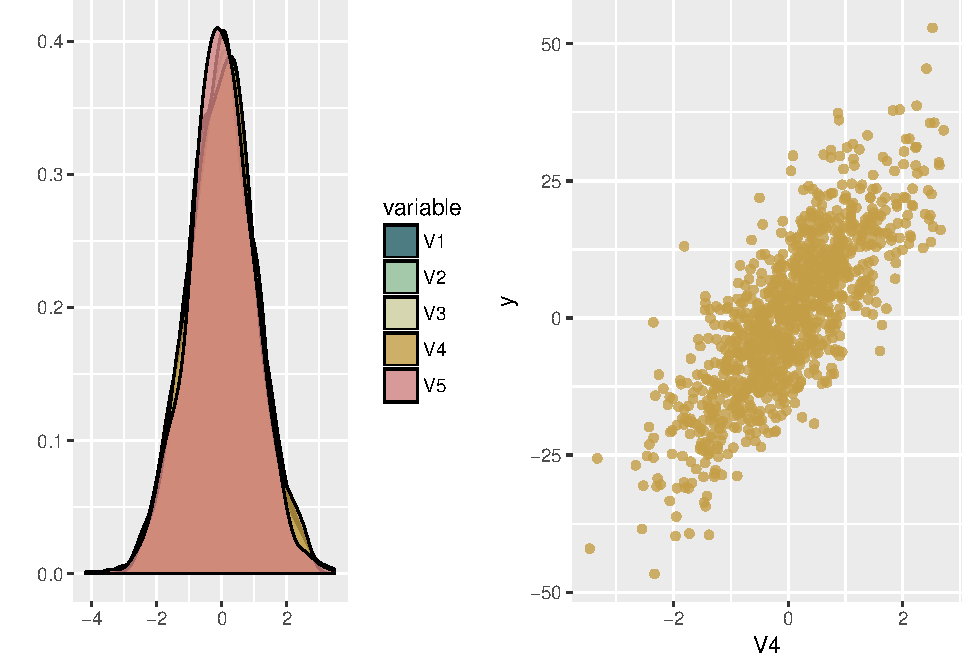
\includegraphics{Thesis_files/figure-latex/figdenv1v5-1.pdf}
  \caption{\label{fig:figdenv1v5}Density Graphs for V1 through V5 and a Plot
  of Y \textasciitilde{} V4, Correlation = .789}
  \end{figure}
  
  ~~~~~ As can be seen in Figure 1 the densities of \(V_1,...,V_5\) are
  all very similar due to the way they were generated.
  
  \section{Models and Comparisons}\label{models-and-comparisons}
  
  \subsubsection{CART: Regression Trees}\label{cart-regression-trees}
  
  \begin{figure}[htbp]
  \centering
  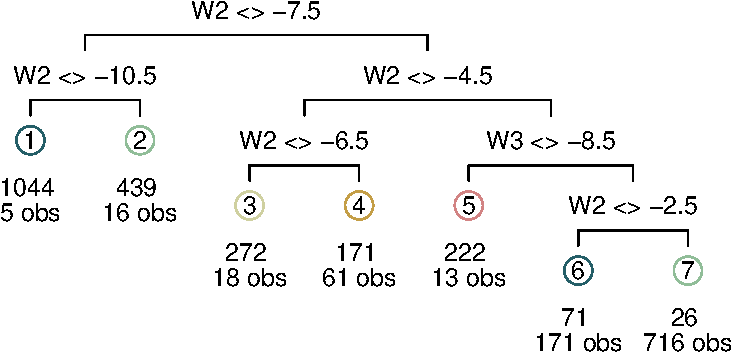
\includegraphics{Thesis_files/figure-latex/figcarts-1.pdf}
  \caption{\label{fig:figcarts}CART for the Model Y\textasciitilde{}, from D1}
  \end{figure}
  
  ~~~~~A single CART tree representing the model \(Y \sim X_1,...,X_{12}\)
  is easy enough to understand. Starting at the very top of the tree,
  predictions can be made based on the values of the leaves (or ending
  nodes) given the requirements of the path to get there. Trees can be
  quite variable, so to get a better idea of the differences between the
  methods let's run a simulation.
  
  \begin{algorithm}
  \caption{Simulation Scheme 2.1}
  \label{sim2.1}
  \begin{algorithmic}[1]
  \For{$i \leq 1000$ }
  \State Randomly sample $\frac 2 3$  of the observations in  $D_1$  to a training set,  $D_{1, train}^i$. The other observations,  $x \in D_1, x \notin D_{1, train}^i$ form the testing set $D_{1, test}^i$
  \State Fit a tree, $T^i$, to the data under the model $Y \sim X_1,...,X_2$ using the observations in      $D_{1}^i$
  \State Calculate the $MSE_{test}$ of the model using the equation:
      $MSE_{test} = \frac 1 n \sum (y_j - \hat{y_j})^2$
  \EndFor
  \end{algorithmic}
  \end{algorithm}
  
  Note that \(n\) is the number of observations in \(D_{1, test}^i\),
  \(y_j \in D_{1, test}^i, \hat{y_j} \in T^i(D_{2, test}^i)\) for
  \(1 \leq j \leq n\) This produces one distribution of \(MSE_{test}\) for
  CART.
  
  \begin{figure}[htbp]
  \centering
  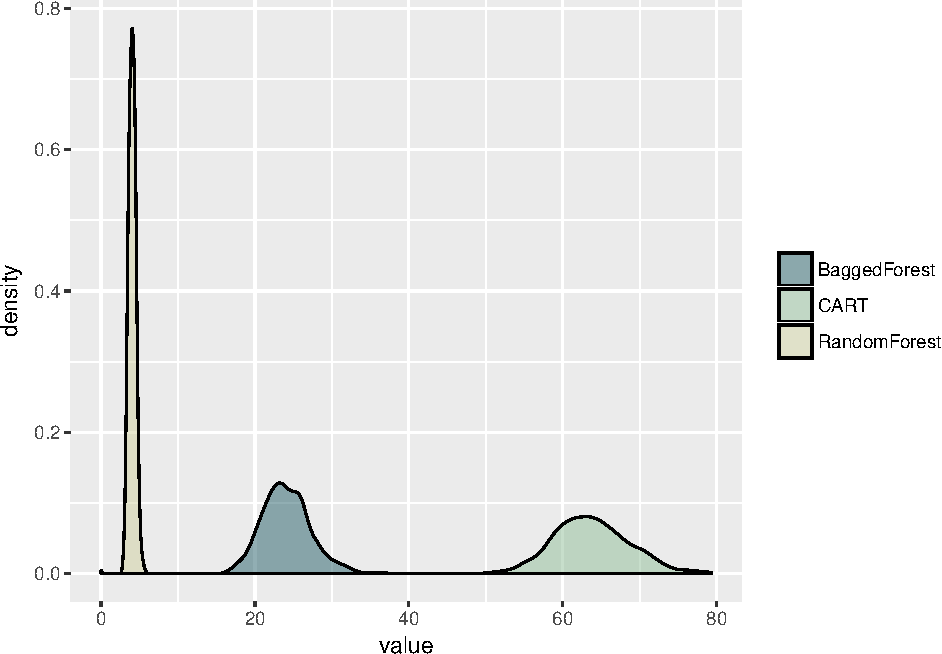
\includegraphics{Thesis_files/figure-latex/baggedvcartvforest-1.pdf}
  \caption{\label{fig:baggedvcartvforest}Simulated MSEtest Distributions of
  CART, Random, and Bagged Forests}
  \end{figure}
  
  ~~~~~The distribution of 100 CART trees' \(MSE_{test}\) in the above
  figure is roughly normal with a variance of \texttt{var(testmseC)}.
  There is a fair amount of variability in a single tree, they are heavily
  dependent on fluctuations in the starting data set. As mention briefly
  in the introduction, bagged forests present one solution to this
  problem. To create a bagged forest, as outlined in \emph{An Introduction
  to Statistical Learning} by James, Witten, Hastie and Tibshirani, 2013,
  many bootstrapped samples are taken from the initial dataset and trees
  are fitted to them. The final predictions are, then, averaged over all
  of the trees. This ensures that while each tree has high variance, when
  they are aggregated the variance will decrease. As one can see, the
  values of \(MSE_{test}\) for the bagged forest were entirely below the
  \(MSE_test\) for the trees and the variance was much smaller. As random
  forests are unbiased, they can be much smaller than their bagged forest
  cousins without sacrificing accuracy.
  
  \chapter{Random Forest Variable
  Importance}\label{random-forest-variable-importance}
  
  \section{Breiman et al Introduce Permuted Variable Importance
  (1984)}\label{breiman-et-al-introduce-permuted-variable-importance-1984}
  
  \subsection{Variable Importance on a Single
  Tree}\label{variable-importance-on-a-single-tree}
  
  ~~~~~Breiman et al in \emph{Classification and Regression Trees} (1984)
  propose a method for variable importance for individual trees that stems
  from their definition of \(\tilde{s}\), a surrogate split. Surrogate
  splits help Brieman et al deal with several common problems: missing
  data, masking, and variable importance. They are defined using logic
  that resembles that behind random forests.
  
  Definitions
  
  ~~~~~Assume the standard structure for tree models. Let \(D\) be the
  dataset composed of \(D = {Y, X_1,...X_p}\), where the model we would
  like to estimate is of the form \(T: Y \sim X_1,...X_p\). For any node
  \(t \in T(D)\), \(s*\) is the best split of the node into daughters
  \(t_r\) and \(t_l\). Take \(X_i \in D\) and let \(S_i\) be the set of
  all of the splits on \(X_i\) in \(T\). Then set \(\bar{S_i}\) equal to
  the complement of \(S_i\), \(\bar{S_i} = S_i^c\). For any possible split
  \(s_i \in S_i \cup \bar{S_i}\), \(s_i\) will split the node \(t\) into
  two daughters, \(t_{i,l}\) and \(t_{i,r}\). Count the number of times
  that \(s*\) and \(s_i\), while splitting differently, generate the same
  left daughter \(t_{l}\) as \(N_{LL}\) and the number of times they
  generate the same right daughter as \(N_{RR}\). Then the probability
  that a case falls within \(t_L \cap t'_L\) is
  \(P(t_L \cap t'_L) = \sum_j \frac{\pi(j) N_j(LL)}{N_j}\) and the
  probability that a case falls within \(t_R \cap t'_R\) is
  \(P(t_R \cap t'_R) = \sum_j \frac{\pi(j) N_j(RR)}{N_j}\). Where
  \(\pi(j)\) is the prior assumed for the the jth variable.Finally, the
  probability that a surrogate split predicts \(s*\) is
  \(P(s*, s_M) = (t_R \cap t'_R) + P(t_L \cap t'_L)\). Then the surrogate
  split is the value of \(s*\) that maximizes this probability. It is
  denoted \(\tilde{s}\)
  
  ~~~~~A surrogate split \(\tilde{s}\),is one that estimates the best
  possible univariate split \(s*\) on node \(t\).
  
  \textbf{Defintion: Variable Importance, Single Tree}
  
  \[VI_{tree}(X_i, T) = \sum_{t \in T} \Delta RSS(\tilde{s_i}, t)\]
  ~~~~~Or the decrease of RSS attributable to \(X_i\) across the tree
  \(T\). In \emph{Classification and Regression Trees},Brieman et al,
  outline several potential problems with this method that the do not
  attempt to solve. First, that this is only one of a number of reasonable
  ways to define variable importance. Second, the variable importances for
  variables \(X_1,..,X_p\) can be effected by outliers or random
  fluctuations within the data. (Ch 5.3)
  
  \subsection{Variable Importance for a Random
  Forest}\label{variable-importance-for-a-random-forest}
  
  ~~~~~One way to define variable importance for a random forest follows
  directly from Breiman et al's definition for a single tree. Recall that
  each tree in a random forest is fit to a bootstrapped sample of the
  original observations. To estimate the test error, therefor, no cross
  validation is needed - each tree is simply tested against the test set
  of observations that were not in that tree's initial training set. To
  determine variable importance for a predictor \(X_j\), we look at the
  RSS of the each tree's prediction that did not split on \(X_j\). These
  values are then averaged over the subset forest that did not include
  \(X_j\). A large value would imply that in trees that included \(X_j\),
  the predictive capabilities were increased.
  
  ~~~~~To formalize that idea, let's refer to the set of trees that did
  not consider \(X_j\), \(T_{x_j}^c\). Now, \(T_{x_j}^c \subset R\), the
  random forest. The subset of the original data that will be tested on
  each tree, \(t\), is \(\bar{B}^t\). The dimensions of \(\bar{B}^t\) are
  \(\nu_t\) x \(p\), where \(p\) is the number of predictors and
  \(\nu \leq n\). The number of trees in \(T_{x_j}^c\) is \(\mu\) where
  \(\mu \leq ntree\)
  
  ~~~~~Now, base variable importance is:
  
  \[VI_{\alpha}(X_j, R) =  \sum_{t \in T_{x_j}^c} \frac 1 {\nu_t} RSS(t,\bar{B}_t)\]
  
  ~~~~~However, this method poses some problems. Namely, while variable
  importance for random forests is more stable than for the variable
  importance values for CART, (this is because the model is less variable
  in general), it is lacking the traditional inferential capabilities of
  other regression models. In an effort to derive a p-value for variable
  importance values, Breiman 2001b, describes a \emph{permuted variable
  importance} or \(VI_{\beta}\) that does not utilize \(T_{x_j}^c\).
  
  \begin{algorithm}
  \caption{Permuted Variable Importance for Random Forests, $VI_{\beta}$}
  \label{breiman}
  \begin{algorithmic}
  \State Fit a random forest, $R$ on the dataset $D$ fitting the model $Y \sim X_1,...,X_p$.
  \For{each $X_i \in {{X_1,...,X_p}}$}
  \For{each $t \in R$}
  \State Calculate: $\Phi_o =  \frac 1 {\nu_t} RSS(t,\bar{B}^t)$
  \State Permute $X_i$. Now find $\Phi^* =  \frac 1 {\nu_t} RSS(t,\bar{B}_t^*)$
  \State The difference between these values, $\Phi^* - \Phi_o$,  is the variable importance for $X_j$ on $t$,  
  \EndFor
  \State Average over all $t \in R$ 
   $$VI_{\beta}(X_j) = \frac 1 {ntree} \sum^{ntree} \Phi^* - \Phi_o$$
   $$VI_{\beta}(X_j) = \frac 1 {ntree} \sum^{ntree} \frac 1 {\nu_t} RSS(t,\bar{B}_t^*) - \frac 1 {\nu_t} RSS(t,\bar{B}^t)$$
  \EndFor
  \end{algorithmic}
  \end{algorithm}
  
  ~~~~~Again, a large variable importance value suggests that \(X_j\) is a
  valuable predictor for the model.
  
  \section{Strobl et al Respond (2008)}\label{strobl-et-al-respond-2008}
  
  ~~~~~Strobl et al (2008) respond to Breiman's method with one main
  argument: the null hypothesis implied by the permutation distribution
  utilized in permuted variable importance is that \(X_i\) is independent
  of \(Y\) \textbf{and} \({X_j \notin X_1,...,X_p}\) so the null
  hypothesis will be rejected in the case where \(X_j\) is independent of
  \(Y\) but not some subset of the other predictors. As correlation among
  the predictors is very common in data sets that are used for random
  forests, this is a large problem for Breiman's method.
  
  ~~~~~To alleviate this difficulty, Strobl et al propose a permutation
  scheme under the null hypothesis that \(X_j\) given it's relationship
  with the other predictors is independent of \(Y\).
  
  \begin{algorithm}
  \caption{Conditional Variable Importance for Random Forests, $VI_{\gamma}$}
  \label{strobl}
  \begin{algorithmic}[1]
  \State Fit a random forest, $R$ on the dataset $D$ fitting the model $Y \sim X_1,...,X_p$.
  \For{each $t \in R$}
  \State Calculate: $\Psi_o =  \frac 1 {\nu_t} RSS(t,\bar{B}^t)$
  \For{each $X_i \in {{X_1,...,X_p}}$}
  \State Select $Z \in X_1,...,X_{i-1}, X_{i+1},...,X_p$ to condition on when permuting $X_j$
  \State Use the cutpoints on each variable in $Z$ to create a grid on $X_j$
  \State Permute $X_j$ with respect to this grid
  \State Now find $\Psi^* =  \frac 1 {\nu_t} RSS(t,\bar{B}_t^*)$
  \State The difference between these values, $\Psi^* - \Psi_o$,  is the variable importance for $X_j$ on $t$,  
  \EndFor
  \State Average over all $t \in R$ 
   $$VI_{\gamma}(X_i,R) = \frac 1 {ntree} \sum^{ntree} \Psi^* - \Psi_o$$
   $$VI_{\gamma}(X_i, R) = \frac 1 {ntree} \sum^{ntree} \frac 1 {\nu_t} RSS(t,\bar{B}_t^*) - \frac 1 {\nu_t} RSS(t,\bar{B}^t)$$
  \EndFor
  \end{algorithmic}
  \end{algorithm}
  
  ~~~~~There are several ways mentioned in ref:@strobl2008 to choose the
  set of predictors \(Z\) to condition \(X_j\) upon. \(Z\) might be chosen
  due to outside theory about the problem or \(Z\) might include every
  \(p-1\) predictor possible. In that paper's simulations section as well
  as in this one's, \(Z\) is chosen as the set of predictors with
  empirical correlation \(\geq .2\)
  
  \chapter{Chapter 4}\label{chapter-4}
  
  \section{INFFORESTS}\label{infforests}
  
  ~~~~~The INFFOREST variable importance is a method of permuted variable
  importance not unlike that of conditionally permuted variable importance
  (Algorthim 3). Permuted variable importance is calculated at the tree
  level, using the partitions on \(X_j\) from a tree created to predict
  the model \(X_j \sim X_1,..., X_{j-1}, X_{j+1},...,X_p\). This auxiliary
  tree is fit by considering all \(p-1\) predictors at each split and so
  may be quite large or quite small depending on the richness of the
  correlation structure around \(X_j\). The auxiliary tree is also fit
  using the OOB sample for the tree at question. If the auxiliary tree
  results in a single leaf, i.e.~there are no splits, then \(X_j\) is
  permuted blindly, without partitions. If the auxiliary tree results in
  two leaves, there will be two partitions on \(X_j\) to permute \(X_j\)
  within, and so on. After permuting \(X_j\) within these partitions, the
  RSS is calculated for that tree using the OOB sample of predictors,
  including the now-permuted \(X_j\). The absolute difference of the RSS
  after permutation and the RSS with the untouched OOB sample is INFFOREST
  variable importance for that tree. Note that for this reason, the
  INFFOREST variable importance is always greater than or equal to zero,
  and is standardized by the max INFFOREST variable importance value given
  by that tree. As the variable importance values are calculated for each
  tree for each variable, once the method is completed there is a
  distribution of potential variable importance values for \(X_j\), one
  for each tree. These distributions may or may not be normal, depending
  on the multicollinearity of the predictors. The INFFOREST variable
  importance algorithm works as follows:
  
  \begin{algorithm}
  \caption{INFForests, $VI_{inf}(R)$}
  \label{infforest}
  \begin{algorithmic}[1]
  \State Fit a random forest, $R$ on the dataset $D$ fitting the model $Y \sim X_1,...,X_p$.
  \For{each $X_i \in {{X_1,...,X_p}}$}
  \For{each $t \in R$}
  \State Calculate: $\Xi_o =  \frac 1 {\nu_t} RSS(t,\bar{B}^t)$
  \State Calculate a tree $T_i$ that predicts $X_i \sim X_1,...,X_{i-1}, X_{i+1},...X_p$ using the subset of the observations used to fit $t$  
  \State Permute the subset of $X_i$ contained in $\bar{B}_t$ with respect to the set of partitions $P_{xi}$ from $T_i$.
  \State Now find $\Xi^* =  \frac 1 {\nu_t} RSS(t,\bar{B}_t^*)$
  \State The difference between these values, $\Xi^* - \Xi_o$,  is the variable importance for $X_i$ on $t$
  \EndFor
  \State Test the null hypothesis that $0$ is the likely value of $\frac 1 {\nu_t} RSS(t,\bar{B}_t^*)$ using the distribution of values of $\Xi^*$ gathered from each tree in $R$
  \EndFor
  \end{algorithmic}
  \end{algorithm}
  
  ~~~~~INFFOREST variable importance operates under the null hypothesis
  that \(Y\) is independent of \(X_J\) given the correlation structure of
  \(X_j\) and the other \(p-1\) predictors, or that the true INFFOREST
  variable importance for \(X_j\) is 0. The alternative hypothesis is that
  \(Y\) and \(X_j\) are not independent given the correlation structure of
  \(X_j\) and the other predictors or that the INFFOREST variable
  importance for \(X_j\) is greater than zero. After INFFOREST values have
  been computed for the entire forest, they are treated as samples from
  the population of possible INFFOREST values for \(X_j\) given the random
  forest \(R_f\), and a significance test can be under the null
  hypothesis.
  
  \section{\texorpdfstring{Implementation In \texttt{INFTREES} and
  Results}{Implementation In INFTREES and Results}}\label{implementation-in-inftrees-and-results}
  
  \subsection{Notes on the
  Implemetation}\label{notes-on-the-implemetation}
  
  ~~~~~Implementing the \texttt{INFFOREST} and therefor the
  \texttt{INFTREES} algorithms, required creating a suite of functions to
  create trees and random forests. The trees are fit following the
  standard two-part CART-like algorithm. \footnote{A brief note on
    uncertainty is needed here. It's true that in this setting we can say
    that \(V_4\) is actually unimportant to understanding \(Y\), but in
    situations with real data this is profoundly more difficult to parse.
    Often like in the social science situations that Morgan and Sonquist
    encountered, the real relationship between correlated predictors is
    complicated and often there is some theoretical backing or other
    insight that is gained to include variables that may not be important
    to the model.} The function chooses a variable to split on with linear
  correlation with respect to \(Y\), but instead of looking for
  correlations above a certain threshold which is common, it chooses the
  variable with the highest correlation when compared to its peers. This
  alleviates the situation where a variable with a non-linear relationship
  would be passed over again and again. The splitting is done via
  minimization of the following function with respect to \(i\):
  
  \[RSS_{node} (i,X,Y) = RSS_{leaf}(Y|X <i) + RSS_{leaf}(Y|X \geq i) \]
  \[RSS_{leaf} = \sum (y - \hat{y})^2 \]
  \[\hat{Y}: \hat{y} \in \hat{Y}: \hat{y} = E(Y), \ where\  |\hat{Y}| = |Y|\]
  
  ~~~~~This function considers the regression case only, and only numeric
  predictors. Leafs are created when the resultant split would be
  unsatisfactory, i.e.~at least one daughter node would have five members
  or less. This generates very large trees - a quality that is not an
  issue in random forests but may be problematic in a stand-alone setting.
  At this time, there is also no function to prune the trees.
  
  \subsubsection{\texorpdfstring{Table 2: A Home-Grown Tree on
  \(Y~X_1+X_2+X_3+X_4\)}{Table 2: A Home-Grown Tree on Y\textasciitilde{}X\_1+X\_2+X\_3+X\_4}}\label{table-2-a-home-grown-tree-on-yx_1x_2x_3x_4}
  
  \begin{tabular}{l|l|l|l|l}
  \hline
  var & n & dev & ypred & split.cutleft\\
  \hline
  X2 & 50 & 5958.56398616138 & -3.32099458459633 & 1.89262782336418\\
  \hline
  leaf & 14 & 1683.79172385909 & 15.2166924465285 & 0\\
  \hline
  X1 & 36 & 1771.9972397028 & -10.5300950967004 & -0.758420438327835\\
  \hline
  X1 & 27 & 1061.15524312941 & -5.71617332730625 & -0.251307488862014\\
  \hline
  leaf & 17 & 720.083908357861 & -2.51280971153014 & 0\\
  \hline
  leaf & 10 & 341.071334771552 & -11.1618914741256 & 0\\
  \hline
  leaf & 9 & 239.837381494473 & -24.971860404883 & 0\\
  \hline
  \end{tabular}
  
  ~~~~~The tree output is read in the following way: each row corresponds
  to a node of the tree which considers \texttt{n} observations. The mean
  of the \(Y\) values included in the node are \texttt{ypred}. If there is
  an optimal and allowable split, \footnote{Another point that could be
    said is that, no \(V_4\) is not unimportant, \(V_1, V_2,\) and \(V_3\)
    are just stand ins for the real star, \(V_4\), as they are nearly the
    same (\(\rho \sim 1\)). Then the real relationship represented here is
    \(Y \sim (5 + 5 + 2) \cdot V_4 + -5 \cdot V_5 + -5 \cdot V_6 + -2 \cdot V_7\).
    This model is not unsuccessful in capturing the structure of the data,
    and this is typically the practice used to model data with highly
    correlated predictors. If this seems philosophically satisfying to
    you, the rest of this thesis may seem a bit inconsequential.} then the
  chosen variable, \texttt{var}, and the \(RSS_{node}\), \texttt{dev}, are
  recorded.\footnote{Recall that we only allow splits to take place that
    split the data into two groups, each with more than five members.} The
  value of the variable in question that acts as the split point is
  recorded as \texttt{split.cutleft}. If there is no split on the node in
  question, then \texttt{var} will be recorded as
  \texttt{\textless{}leaf\textgreater{}} and the \texttt{dev} value will
  be the value of \(RSS_{leaf}\) at this node.
  
  ~~~~~The tree output is read roughly from top to bottom, with a coda in
  the middle. The first row corresponds to the first node, or the node
  that includes the entire dataset. The second row is the beginning of the
  right subtree or the right daughter of first node. This pattern
  continues, favoring the right daughter, until a leaf is reached. The
  left daughter of the first node is found after all of the splits off of
  the right daughter have finished but is easily identified as the row
  with a value of \texttt{n} that is exactly the difference between the
  \texttt{n} values of the first two rows. In the case where the right
  daughter contained many more observations of the original dataset, there
  may be a node within the right subtree that contains the same number of
  observations as the left daughter of the first node. In this case, the
  left daughter is simply the second row with this property. The pattern
  of following the right daughter until a leaf is reached continues with
  the left subtree.
  
  ~~~~~The INFTREE function follows the algorithm referenced earlier. The
  partitions on \(X_j\) are generated by fitting a tree, \(T\), to the
  model \(X_j \sim X_1,..., X_{j-1}, X_{j+1},..X_p\) and calculating the
  predictions \(T(X_1,..., X_{j-1}, X_{j+1},..X_p)\). Then permuting
  \(X_j\) with respect to the partitions on \(X_j\) given by those
  predictions. For example, if \(x_j \in X_j\) and the value of
  \(T(x_1,..., x_{j-1}, x_{j+1},..x_p)\) corresponding to \(x_j\) is
  \(\alpha\), \(x_j\) is permuted along with the other values of \(X_j\)
  that also have \(T(x_1,..., x_{j-1}, x_{j+1},..x_p)\) corresponding to
  \(\alpha\).
  
  ~~~~~The values of \(INFFOREST(X_j)\) are scaled in the following way:
  since the INFFOREST function computes the INFFTREES, (or the difference
  in post and pre permutation RSS), values in a tree-wise manner, each
  tree's values are divided by the maximum value. This ensures that the
  values are between zero and one, and that in each tree one variable is
  clearly deemed the \emph{most important}.
  
  \subsection{Results}\label{results}
  
  \begin{figure}[htbp]
  \centering
  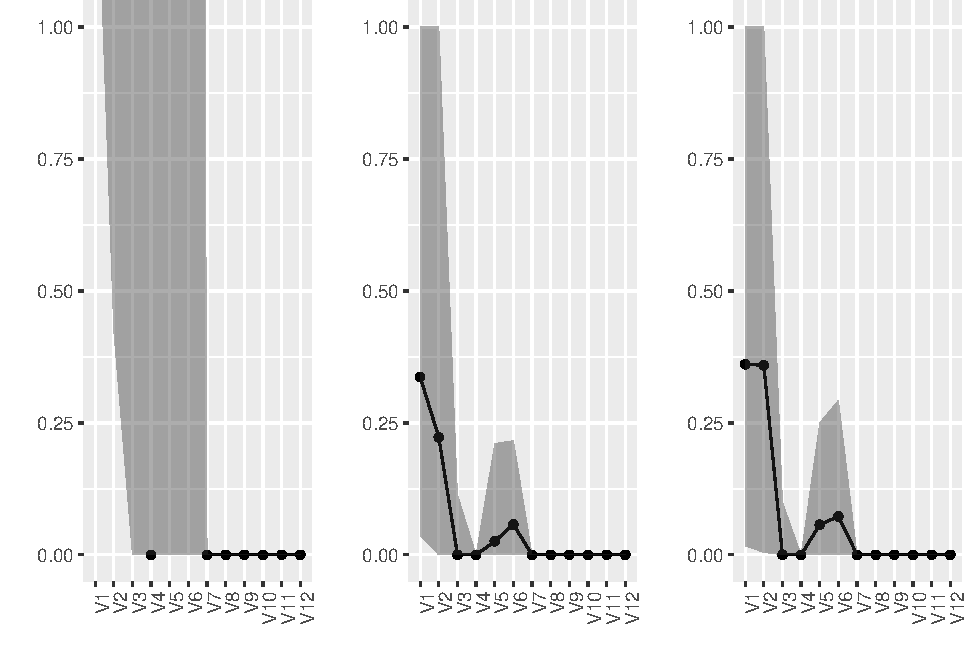
\includegraphics{Thesis_files/figure-latex/figmtry-1.pdf}
  \caption{\label{fig:figmtry}Median Values of INFFOREST Variable Importance
  for mtry = 4,6 and 8}
  \end{figure}
  
  As in (ref Strobl et al 2008), the median INFFOREST variable importance
  scores are reported here for the dataset \(D_1\). \footnote{It's the
    convention to call the \(RSS_{node}\) the deviance at a node \(N\),
    but, of course, this only makes sense when the node is a leaf.}
  
  As noted in several publications (Strobl et al, Breiman, Intro to Stat
  Learning), random forests structure is dependent on the value of
  \texttt{mtry}.\footnote{A great deal of effort was undertaken by the
    author to find the definitive, authentic CART algorithm. This
    implementation follows the rough strokes set out in the 1984 text
    \emph{Classification and Regression Trees} to the best of the author's
    ability and may not be exactly the algorithm found in R packages like
    `tree()'} INFFOREST variable importance remains fairly consistent as
  \texttt{mtry} fluctuates.
  
  \chapter{INFFOREST Comparisons With Other
  Methods}\label{infforest-comparisons-with-other-methods}
  
  \begin{figure}[htbp]
  \centering
  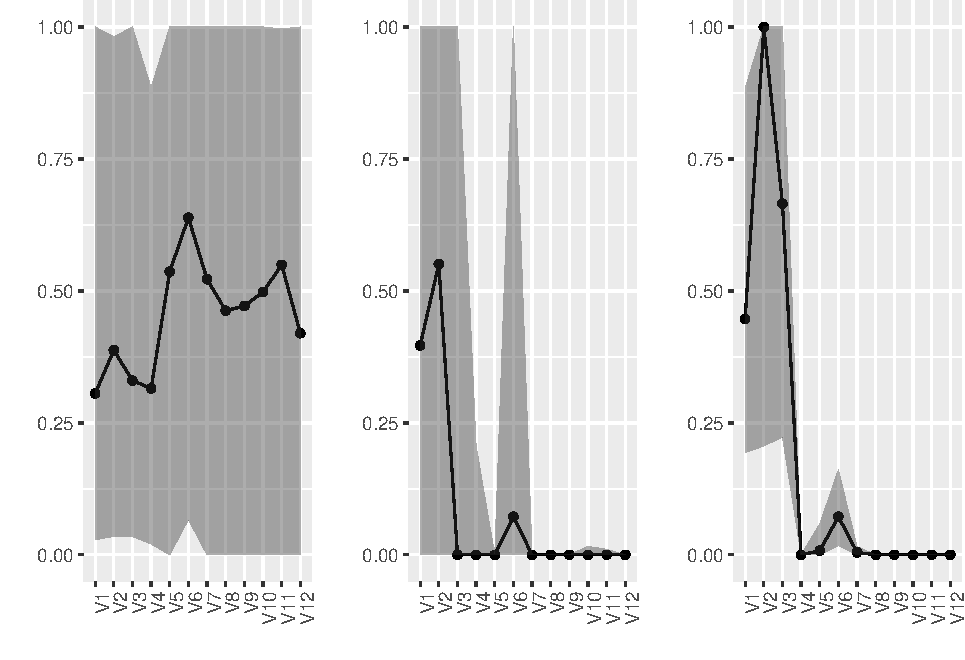
\includegraphics{Thesis_files/figure-latex/figcomparisons-1.pdf}
  \caption{\label{fig:figcomparisons}Median Values of INFFOREST, Conditionally
  Permuted, and Permuted Variable Importance}
  \end{figure}
  
  INFFOREST holds its own amongst the other methods described in Chapter
  4. The conditional permuted variable importance, when ran on the same
  random forest, had more difficulty parsing out the situation with paired
  variables than INFFOREST, only selecting the first two variables to be
  important. Permuted variable importance does not pick up on the
  correlation structure within the predictors and deems \(V2\) and \(V6\)
  unimportant.
  
  INNFOREST and conditional permuted variable importance both ignored the
  unfluential predictors that were not correlated with \(V1,V2,V3\) and
  \(V4\). This is a situation that also occured in the simulation run in
  Strobl et al (2008b).


  % Index?

\end{document}
